\section{Neutral binary qualification with fixed CO2--water induced association}

\subsection{Question and conditions}

The practical neutral stage asks which source-backed MEA association family
transfers between the two Cai MEA--water pressure levels under fixed Held 2B
water, and whether the source CO2--water interaction reproduces the independent
Kiepe coexistence data. These calculations precede the nine-species reactive
fit; no ionic or reaction parameter is estimated here.

\subsection{Methods and sources}

The MEA--water calculation fits one $k_{\mathrm{MEA,H2O}}$ on the
\SI{101.33}{\kilo\pascal} Cai series and evaluates the independent
\SI{66.66}{\kilo\pascal} series. It compares the Baygi 2B, 3B, and 4C MEA
families under the same Held water family. All 25 states use component
log-fugacity closure and exact Engine derivatives checked against centered
finite differences.

The CO2--water calculation uses all 39 nonzero-composition rows from Kiepe
et al. (2002), Table 1, DOI \href{https://doi.org/10.1021/ie020154i}{10.1021/ie020154i}.
The molecular, association, and temperature-dependent binary parameters are
from Pabsch et al. (2020), Tables 2 and 6, DOI
\href{https://doi.org/10.1021/acs.jced.0c00704}{10.1021/acs.jced.0c00704}.
The calculation uses the declared liquid and incipient-vapor topology.

\subsection{Results}

\begin{table}[ht]
\centering
\caption{MEA--water family comparison. Log-RMSE is based on the natural-log
fugacity-closure residual.}
\begin{tabular}{lrrrr}
\toprule
MEA family & $k_{\mathrm{MEA,H2O}}$ & Fit log-RMSE & Held log-RMSE & Held factor \\
\midrule
2B & -0.058566 & 0.06883 & 0.15891 & 1.172 \\
3B & -0.019567 & 0.05900 & 0.11123 & 1.118 \\
4C & -0.036274 & 0.05244 & 0.12577 & 1.134 \\
\bottomrule
\end{tabular}
\end{table}

The 3B family gives the best pressure-level transfer and is retained. For
CO2--water, all 39 states evaluate. The log-pressure RMSE is 0.21228 and the
median multiplicative error is 1.1703. The largest pressure and
chemical-potential residuals are $2.36\times10^{-9}$ and
$1.85\times10^{-8}$, respectively.

\begin{figure}[ht]
\centering
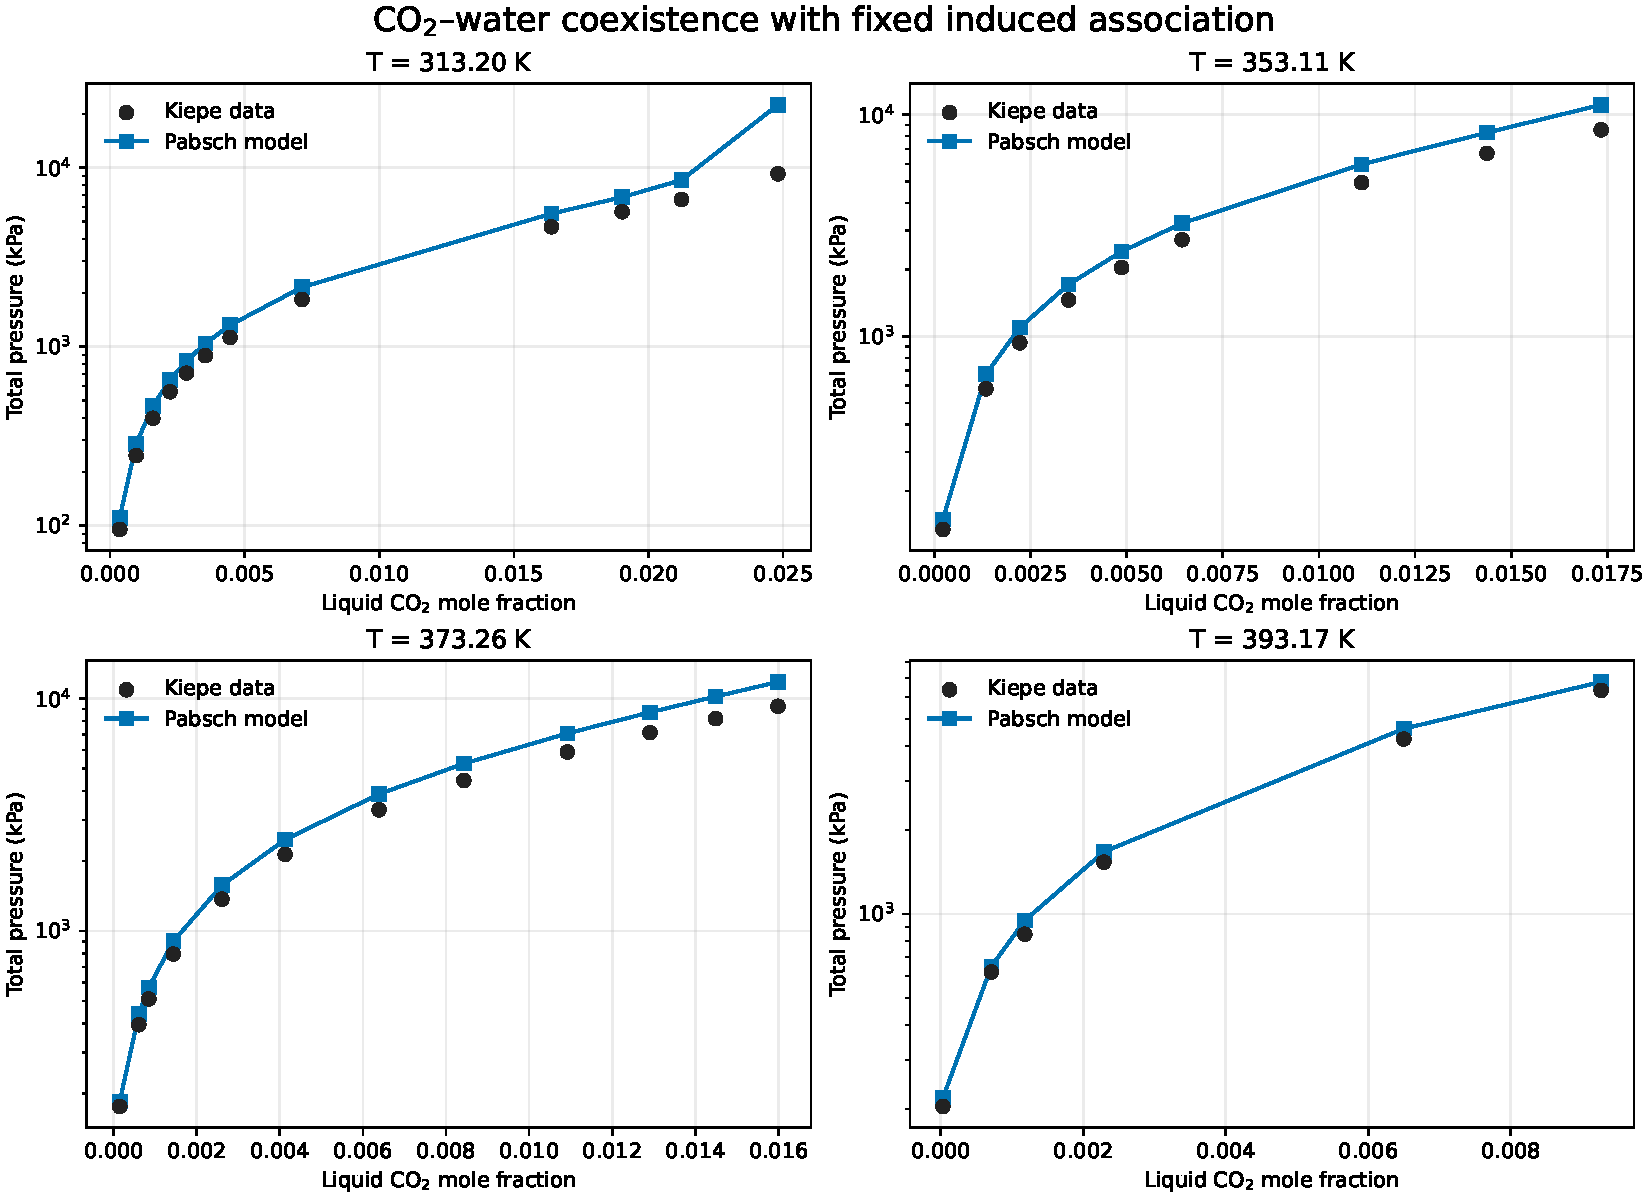
\includegraphics[width=0.96\textwidth]{analyses/phase3/ionic_epcsaft_regression/co2_water_induced_association/figures/co2_water_induced_association.pdf}
\caption{Kiepe observations and the source Pabsch CO2--water calculation at
four temperatures. Exact plotted rows are retained with the analysis.}
\end{figure}

\subsection{Interpretation and limitations}

The evidence supports freezing the Held-water/3B-MEA neutral family and the
source CO2--water temperature correlation before the electrostatic comparison.
The MEA--water source reports composition resolution rather than a statistical
covariance model, so the raw log closure and pressure-level transfer are more
informative than the stringent resolution-normalized gate. The CO2--water
comparison reproduces the same data family used in the source
parameterization; it establishes faithful implementation and practical
agreement, not independent reserved validation. Neither binary calculation
identifies ionic, reaction, or reactive-pressure parameters.

The exact inputs and outputs are linked from the pressure-first and CO2--water
analysis READMEs.
